\documentclass[aspectratio=169, 11pt]{beamer}

\usepackage[english]{babel}
\usepackage[T1]{fontenc}
\usepackage[utf8]{inputenc}
\usepackage{graphicx}
\usepackage{booktabs}
% Shared macros (copied from ../setup.tex)
\newcommand{\app}{\;}                                  % spacing for bare variable juxtaposition
\newcommand{\appexp}{\,}                                % narrower spacing used inside \iexp
\newcommand{\iexp}[1]{\appexp\text{\ttfamily #1}\appexp} % Isabelle-style expression, e.g. a \iexp{+} b
% Labelled underbrace shown only on the given overlay(s), e.g. \ubr{2}{content}{label}.
% \smash[b] discards the depth of the brace, so it is placed directly under its content
% regardless of other braces. Use \ubrspace once per formula to reserve the vertical space.
\usepackage{mathtools} % for \mathclap
% \mathclap makes the label take no width, so it does not affect the formula spacing
\newcommand{\ubrbox}[2]{\underbrace{#1}_{\mathclap{\textit{#2}}}}
\newcommand{\ubr}[3]{\alt<#1>{\smash[b]{\ubrbox{#2}{#3}}}{#2}}
\newcommand{\ubrspace}{\vphantom{\ubrbox{\mathstrut}{\strut}}}
% Like \ubr, but marks a single symbol with a label below an up arrow instead of a brace.
\newcommand{\uarr}[3]{\alt<#1>{\smash[b]{\underset{\mathclap{\substack{\uparrow\\\textit{#3}}}}{#2}}}{#2}}

% Isabelle code listings (copied from ../setup.tex)
\usepackage{listings} % to include code
\usepackage{tcolorbox} % to frame Isabelle code with rounded corners
\tcbuselibrary{listings,skins,breakable}

% Isabelle setup is heavily inspired/partially copy-paste from
% https://github.com/lammich/isabelle_llvm/blob/master/papers/2021_Enschede_Talk/lstisabelle.tex

\lstdefinelanguage{Isabelle}{%
keywords=[1]{theory,begin,end,imports,keywords},
keywords=[2]{fun,datatype,type_synonym,record,
		abbreviation,notation,class,instance,context,interpretation,
		sublocale,global_interpretation,inductive,coinductive,
		primrec,primcorec,typedef,setup,declare,
		lemma,theorem,corollary,proposition,conjecture,example,
		value,export_code},
keywords=[3]{proof,qed,by,done,apply,
		have,show,assume,obtain,let,fix,
		from,with,using,unfolding,
		also,finally,ultimately,next,case,then,hence,thus,and,where},
keywords=[4]{auto,simp,blast,force,fastforce,clarify,clarsimp,
		rule,erule,drule,frule,intro,elim,
		induction,induct,cases,
		subst,unfold,arith,omega,linarith,algebra,metis,meson,transfer},
sensitive=true,
morecomment=[s]{(*}{*)},
morecomment=[l]{--},
% "\<comment>" is rewritten to the classic Isar "--" comment marker by
% scripts/prepare-isabelle-listings.sh before the file reaches listings:
% listings cannot recognize a genuine multi-byte Unicode character (e.g. an
% em dash) as a comment delimiter, and it cannot use `literate` to
% substitute the display text of a string that is itself a delimiter.
morestring=[b]",
literate=
	% {'}{{${}^\prime\!$}}1
	{\%}{{$\lambda$}}1
{\\\%}{{$\lambda$}}1
{\\\$}{{$\mathbin{\,\$\,}$}}1
{->}{{$\rightarrow$}}1
{<-}{{$\leftarrow$}}1
{<.}{{$\langle$}}1
{.>}{{$\rangle$}}1
{<=}{{$\le$}}1
{>=}{{$\ge$}}1
{<->}{{$\leftrightarrow$}}1
{-->}{{$\longrightarrow$}}2
{<-->}{{$\longleftrightarrow$}}1
{=>}{{$\Rightarrow$}}1
{==}{{$\equiv$}}2
{==>}{{$\implies$}}2
{<=>}{{$\Leftrightarrow$}}1
{~=}{{$\ne$}}1
{|}{{$\mid$}}1
{-`}{{$\rightharpoonup$}}1
{|`}{{$\restriction$}}1
{!!}{{$\bigwedge$}}1
{(}{{$($}}1
{)}{{$)$}}1
{\{}{{$\{$}}1
{\}}{{$\}$}}1
{[}{{$[$}}1
{]}{{$]$}}1
{[|}{{$\llbracket$}}1
{|]}{{$\rrbracket$}}1
{\\<lbrakk>}{{$\lsem$}}1
{\\<rbrakk>}{{$\rsem$}}1
{|-}{{$\vdash$}}1
{|=}{{$\models$}}1
{|->}{{$\mapsto$}}1
{|_|}{{$\bigsqcup$}}1
{...}{{$\dots$}}1
{\\x}{{$\times$}}1
{_0}{{${}_0$}}1
{_1}{{${}_1$}}1
{_2}{{${}_2$}}1
{_3}{{${}_3$}}1
{_4}{{${}_4$}}1
{_5}{{${}_5$}}1
{_6}{{${}_6$}}1
{_7}{{${}_7$}}1
{_8}{{${}_8$}}1
{_9}{{${}_9$}}1
{_L}{{${}_L$}}1
{\\_n}{{${}_n$}}1
{\\_i}{{${}_i$}}1
{\\_j}{{${}_j$}}1
{\\_x}{{${}_x$}}1
{\\_y}{{${}_y$}}1
{\\impl}{{${}_\dagger$}}1
{^*}{{$^*$}}1
{^k}{{$^k$}}1
{^d}{{$^d$}}1
{\\<^sup>*}{{$^*$}}1
{\\<^sub>*}{{$_*$}}1
{\\<^sub>A}{{$_A$}}1
{\\<^sub>r}{{$_r$}}1
{\\<^sub>a}{{$_a$}}1
{:_i}{{$:_i$}}1
{\\<A>}{{$\mathcal{A}$}}1
{\\<O>}{{\sf o}}1
{\\<Phi>}{{$\Phi$}}1
{\\<Psi>}{{$\Psi$}}1
{\\<sigma>}{{$\sigma$}}1
{\\<cdot>}{{$\cdot$}}1
{\\<in>}{{$\in$}}1
{\\<le>}{{$\le$}}1
{\\<noteq>}{{$\ne$}}1
{\\<lambda>}{{$\lambda$}}1
{\\<longrightarrow>}{{$\longrightarrow$}}1
{\\<longleftrightarrow>}{{$\longleftrightarrow$}}1
{\\<Rightarrow>}{{$\Rightarrow$}}1
{\\<Longrightarrow>}{{$\Longrightarrow$}}1
{\\<rightarrow>}{{$\rightarrow$}}1
{\\<leftarrow>}{{$\leftarrow$}}1
{\\<mapsto>}{{$\mapsto$}}1
{\\<equiv>}{{$\equiv$}}1
{\\<and>}{{$\wedge$}}1
{\\<or>}{{$\vee$}}1
{\\<And>}{{$\bigwedge$}}1
{\\<Up>}{{$\Uparrow$}}1
{\\<Down>}{{$\Downarrow$}}1
{\\<Union>}{{$\bigcup$}}1
{\\<up>}{{$\uparrow$}}1
{\\<down>}{{$\downarrow$}}1
{\\<times>}{{$\times$}}1
{\\<forall>}{{$\forall$}}1
{\\<exists>}{{$\exists$}}1
{\\<nexists>}{{$\nexists$}}1
{\\<union>}{{$\cup$}}1
{\\<inter>}{{$\cap$}}1
{\\<subset>}{{$\subset$}}1
{\\<subseteq>}{{$\subseteq$}}1
{\\<supset>}{{$\supset$}}1
{\\<supseteq>}{{$\supseteq$}}1
{\\<alpha>}{{$\alpha$}}1
{\\<beta>}{{$\beta$}}1
{\\<gamma>}{{$\gamma$}}1
{\\alpha}{{$\alpha$}}1
{\\beta}{{$\beta$}}1
{\\gamma}{{$\gamma$}}1
{\\<Gamma>}{{$\Gamma$}}1
{\\<langle>}{{$\langle$}}1
{\\<rangle>}{{$\rangle$}}1
{\\<not>}{{$\neg$}}1
{\\<box>}{{$\oblong$}}1
{\\<bot>}{{$\bot$}}1
{\\<top>}{{$\top$}}1
{\\<notin>}{{$\notin$}}1
{\\<guillemotright>}{{$\gg$}}1
{\\in}{$\in$}1
{\\and}{$\wedge$}1
{\\or}{$\vee$}1
{\\Phi}{{$\Phi$}}1
{\\Psi}{{$\Psi$}}1
{\\le}{{$\le$}}1
{\\Up}{{$\Uparrow$}}1
{\\Down}{{$\Down$}}1
{>>}{{$\gg$}}1
{>>=}{{${\gg}{=}$}}1
{<*lex*>}{{$\times_{\sf lex}$}}1
{\\<open>}{{\rm\guilsinglleft}}1
{\\<close>}{{\rm\guilsinglright}}1,
}

\lstdefinestyle{isabellestyle}{%
	language=Isabelle,
	basicstyle={\ttfamily},
	columns=[c]fullflexible,
	keywordstyle=[1]\rm\ttfamily\fontseries{b}\color{cd_blue},
	keywordstyle=[2]\rm\ttfamily\fontseries{m}\color{cd_additional_green_100_percent},
	keywordstyle=[3]\rm\ttfamily\fontseries{b}\color{cd_additional_brown_100_percent},
	keywordstyle=[4]\rm\ttfamily\fontseries{b}\color{cd_additional_pink_100_percent},
	commentstyle=\color{gray}\itshape,
	stringstyle=\color{cd_additional_brown_100_percent},
	breaklines=true,
	breakatwhitespace=true,
	showstringspaces=false,
	captionpos=b,
	aboveskip=0pt,
	belowskip=0pt,
	keepspaces=true,
}

% Framing (border, rounded corners, background, inner margin) is handled by
% the tcolorbox around the listing, not by the listings package itself.
\tcbset{
	isabellebox/.style={
			enhanced,
			listing only,
			listing remove caption=false,
			colback=cd_background_sand_50_percent,
			colframe=cd_blue,
			boxrule=0.4pt,
			arc=2mm,
			boxsep=0pt,
			left=1em,
			right=1em,
			top=0.6em,
			bottom=0.6em,
			unbreakable,
		}
}

\lstdefinestyle{isabelleinline}{%
	language=Isabelle,
	basicstyle=\ttfamily,
	columns=[c]fullflexible,
	keywordstyle=[1]\rm\ttfamily\fontseries{b}\color{cd_blue},
	keywordstyle=[2]\rm\ttfamily\fontseries{m}\color{cd_additional_green_100_percent},
	keywordstyle=[3]\rm\ttfamily\fontseries{b}\color{cd_additional_brown_100_percent},
	keywordstyle=[4]\rm\ttfamily\fontseries{b}\color{cd_additional_pink_100_percent},
	commentstyle=\color{gray}\itshape,
	stringstyle=\color{cd_additional_brown_100_percent},
	showstringspaces=false,
	keepspaces=true,
	% backgroundcolor=\color{cd_additional_sand_50_percent},
}
\newcommand{\inlinecode}{\lstinline[style=isabelleinline]}
\newtcblisting{isabellecode}[1][]{%
	isabellebox,
	listing options={style=isabellestyle,#1},
}

% Pseudocode listings (copied from ../setup.tex)
\lstdefinelanguage{Pseudocode}{%
sensitive=true,
morecomment=[l]{//},
literate=
	{<-}{{$\leftarrow$}}1
{->}{{$\rightarrow$}}1,
}

\lstdefinestyle{pseudocodestyle}{%
	language=Pseudocode,
	basicstyle={\ttfamily},
	columns=[c]fullflexible,
	commentstyle=\color{gray}\itshape,
	breaklines=true,
	breakatwhitespace=true,
	showstringspaces=false,
	aboveskip=0pt,
	belowskip=0pt,
	keepspaces=true,
}

\newtcblisting{pseudocode}[1][]{%
	isabellebox,
	listing options={style=pseudocodestyle,#1},
}



% Speaker notes as PDF text annotations (shown in the pympress Annotations view).
% Only emitted when built through main-notes.tex (see build.sh), so main.pdf stays clean.
\ifdefined\withnotes
  % pdfcomment loads datetime2, which changes the format of \today; restore the original
  \let\origtoday\today
  \usepackage{pdfcomment}
  \let\today\origtoday
  \newcommand{\spnote}[1]{\pdfcomment[icon=Note,color=yellow,opacity=1]{#1}}
\else
  \newcommand{\spnote}[1]{}
\fi


% Bibliography: same sources as the thesis (see ../setup.tex)
\usepackage[backend=bibtex,style=numeric,sorting=none]{biblatex}
\addbibresource{../references/motivation.bib}
\addbibresource{../references/fundamentals.bib}
\addbibresource{../references/methodology.bib}
\addbibresource{../references/multiprecision.bib}
\addbibresource{../references/datatypes.bib}
\addbibresource{../references/evaluation.bib}
\addbibresource{../references/discussion.bib}

% Concise bibliography: keep author, title, venue, and year only
\DeclareFieldFormat{labelnumberwidth}{\mkbibbrackets{#1}}
\AtEveryBibitem{%
  \clearfield{url}\clearfield{urldate}\clearfield{doi}\clearfield{isbn}\clearfield{issn}%
  \clearfield{eprint}\clearfield{note}\clearfield{pages}\clearfield{series}%
  \clearfield{volume}\clearfield{number}\clearfield{abstract}%
  \clearlist{publisher}\clearlist{location}\clearlist{address}\clearlist{organization}%
  \clearname{editor}}
\setbeamerfont{bibliography entry author}{size=\scriptsize}
\setbeamerfont{bibliography entry title}{size=\scriptsize}
\setbeamerfont{bibliography entry location}{size=\scriptsize}
\setbeamerfont{bibliography entry note}{size=\scriptsize}
\usepackage{tikz}
\usepackage{appendixnumberbeamer} % appendix frames are excluded from the total slide count
\usetikzlibrary{circuits.logic.US, positioning, calc, shapes.multipart, arrows.meta}
\newcommand{\tikzmark}[1]{\tikz[remember picture, overlay]\node[coordinate] (#1) {};}

\usetheme{CambridgeUS}
\setbeamertemplate{navigation symbols}{}

% Colors from Corporate Design Uni Freiburg (same as ../setup.tex)

\definecolor{cd_blue}{HTML}{344A9A}
\definecolor{cd_black}{HTML}{000000}
\definecolor{cd_white}{HTML}{FFFFFF}

\definecolor{cd_background_blue_100_percent}{HTML}{344A9A}
\definecolor{cd_background_blue_80_percent}{HTML}{5D6BAD}
\definecolor{cd_background_blue_60_percent}{HTML}{868DC2}
\definecolor{cd_background_blue_40_percent}{HTML}{AFB1D8}
\definecolor{cd_background_blue_20_percent}{HTML}{D7D8EC}
\definecolor{cd_background_dark_blue}{HTML}{00004a}
\definecolor{cd_background_sand_100_percent}{HTML}{f6f1e3}
\definecolor{cd_background_sand_50_percent}{HTML}{faf8f1}

\definecolor{cd_additional_green_100_percent}{HTML}{00a082}
\definecolor{cd_additional_green_80_percent}{HTML}{27b29b}
\definecolor{cd_additional_green_60_percent}{HTML}{7bc6b4}
\definecolor{cd_additional_green_40_percent}{HTML}{afdace}
\definecolor{cd_additional_green_20_percent}{HTML}{daede7}
\definecolor{cd_additional_brown_100_percent}{HTML}{8f6b30}
\definecolor{cd_additional_brown_80_percent}{HTML}{a58959}
\definecolor{cd_additional_brown_60_percent}{HTML}{bca683}
\definecolor{cd_additional_brown_40_percent}{HTML}{d2c4ac}
\definecolor{cd_additional_brown_20_percent}{HTML}{e9e1d6}
\definecolor{cd_additional_yellow_100_percent}{HTML}{ffe863}
\definecolor{cd_additional_yellow_80_percent}{HTML}{ffed82}
\definecolor{cd_additional_yellow_60_percent}{HTML}{fff1a1}
\definecolor{cd_additional_yellow_40_percent}{HTML}{fff6c1}
\definecolor{cd_additional_yellow_20_percent}{HTML}{fffae0}
\definecolor{cd_additional_pink_100_percent}{HTML}{f5c2ed}
\definecolor{cd_additional_pink_80_percent}{HTML}{f7cef1}
\definecolor{cd_additional_pink_60_percent}{HTML}{f9daf4}
\definecolor{cd_additional_pink_40_percent}{HTML}{fbe7f8}
\definecolor{cd_additional_pink_20_percent}{HTML}{fdf3fb}

% Replace the dark red of the CambridgeUS (beaver) color theme with the CD colors

\setbeamercolor{structure}{fg=cd_blue}
\setbeamercolor{normal text}{fg=cd_black, bg=cd_white}
\setbeamercolor{alerted text}{fg=cd_additional_green_100_percent}
\setbeamercolor{section in toc}{fg=cd_black, bg=cd_white}

\setbeamercolor*{palette primary}{fg=cd_white, bg=cd_background_blue_80_percent}
\setbeamercolor*{palette secondary}{fg=cd_white, bg=cd_additional_green_100_percent}
\setbeamercolor*{palette tertiary}{fg=cd_white, bg=cd_blue}
\setbeamercolor*{palette quaternary}{fg=cd_white, bg=cd_blue}

\setbeamercolor*{sidebar}{fg=cd_white, bg=cd_blue}
\setbeamercolor*{palette sidebar primary}{fg=cd_black}
\setbeamercolor*{palette sidebar secondary}{fg=cd_white}
\setbeamercolor*{palette sidebar tertiary}{fg=cd_blue}
\setbeamercolor*{palette sidebar quaternary}{fg=cd_background_blue_20_percent}

\setbeamercolor{titlelike}{fg=cd_white, bg=cd_blue}
\setbeamercolor{frametitle}{fg=cd_white, bg=cd_blue}
\setbeamercolor{frametitle right}{bg=cd_additional_green_100_percent}

\setbeamercolor{block title}{fg=cd_white, bg=cd_blue}
\setbeamercolor{block body}{fg=cd_black, bg=cd_background_blue_20_percent}
\setbeamercolor{block title alerted}{fg=cd_white, bg=cd_additional_green_100_percent}
\setbeamercolor{block body alerted}{fg=cd_black, bg=cd_additional_green_20_percent}
\setbeamercolor{block title example}{fg=cd_white, bg=cd_additional_brown_100_percent}
\setbeamercolor{block body example}{fg=cd_black, bg=cd_additional_brown_20_percent}

\title[Pastèque with Arbitrarily Large Integers]{Pastèque, the verified PAC Checker in Isabelle-LLVM with Arbitrarily Large Integers}
\subtitle{Master's Thesis}
\author{Milan Müller}
\institute[Uni Freiburg]{Albert-Ludwigs-Universität Freiburg}
\date{\today}

\begin{document}

\begin{frame}
  \titlepage
\end{frame}

\section{The Practical Algebraic Calculus}

\subsection{Motivation}

% \begin{frame}
%     \begin{itemize}
%         \item SAT can verify (large) adders
%         \item Does not scale for multipliers \cite{Kaufmann-column-wise-verification}
%         \item BDDs also do not scale
%         \item $\rightsquigarrow$ use algebraic reasoning
%     \end{itemize}
% \end{frame}

\begin{frame}{Example: OR from AND and NOT}
    \setbeamercovered{invisible}
    \centering
    \begin{tikzpicture}[circuit logic US, node distance=0.8cm,
        lbl/.style={font=\small, fill=white, inner sep=1pt}]
        % inputs
        \node (a) at (0, 1) {$a$};
        \node (b) at (0, -1) {$b$};
        % negation gates
        \node[not gate, draw, anchor=input] (g1) at (1.2, 1) {};
        \node[not gate, draw, anchor=input] (g2) at (1.2, -1) {};
        % and gate
        \node[and gate, draw, logic gate inputs=nn, anchor=input 1] (g3) at (3, 0.1) {};
        % output negation
        \node[not gate, draw, anchor=input] (g4) at (6, 0) {};
        \node (s) at (9, 0) {$s$};

        \draw (a) -- (g1.input);
        \draw (b) -- (g2.input);
        \draw (g1.output) -- node[lbl, above] {$n_1$} ++(0.6,0) |- (g3.input 1);
        \draw (g2.output) -- node[lbl, below] {$n_2$} ++(0.6,0) |- (g3.input 2);
        \draw (g3.output) -- node[lbl, above] {$n_3$} (g4.input);
        \draw (g4.output) -- (s);

    \end{tikzpicture}
    \begin{alignat*}{6}
        \tikzmark{tl1}0 &= -a + 1 - n_1   \qquad\qquad & \tikzmark{tl2}\uncover<2->{0} & \uncover<2->{{}= a^2 - a} \qquad\qquad & \uncover<2->{0} & \uncover<2->{{}= n_1^2 - n_1}\\
        0 &= -b + 1 - n_2   \qquad\qquad & \uncover<2->{0} & \uncover<2->{{}= b^2 - b} \qquad\qquad & \uncover<2->{0} & \uncover<2->{{}= n_2^2 - n_2}\\
        0 &= -n_3 + n_1 n_2\tikzmark{br1} \qquad\qquad & \uncover<2->{0} & \uncover<2->{{}= s^2 - s} \qquad\qquad & \uncover<2->{0} & \uncover<2->{{}= n_3^2 - n_3}\tikzmark{br2}\\
        0 &= -n_3 + 1 - s\tikzmark{bl}   &   &            &   &
    \end{alignat*}
    \begin{tikzpicture}[remember picture, overlay, box/.style={thick, rounded corners}]
        \coordinate (mid1) at ($(tl1)!.5!(br1)$);
        \coordinate (mid2) at ($(tl2)!.5!(br2)$);
        \draw<3->[box] ($(tl1)+(-6pt,13pt)$) rectangle ($(br1 |- bl)+(8pt,-7pt)$);
        \node<3->[anchor=north] at ($(mid1 |- bl)+(0,-9pt)$) {$P$};
        \draw<3->[box] ($(tl2)+(-6pt,13pt)$) rectangle ($(br2 |- bl)+(8pt,-7pt)$);
        \node<3->[anchor=north] at ($(mid2 |- bl)+(0,-9pt)$) {$B(X)$};
    \end{tikzpicture}
\end{frame}

\begin{frame}
    \begin{itemize}
        \item Roots $\sim$ gate-level semantics (possible assignments)
        \item Consider ideal $\langle P \cup B(X) \rangle$
        \item Specification $f :\equiv 0 = -s + a + b -ab$
        \item Check: $f \mathrel{\overset{?}{\in}} \langle P \cup B(X) \rangle$
        \item AMulet \cite{amulet2}: Decide ideal membership + PAC certificate \cite{pac-2018, pac-2024}
        \item Pacheck/Pastèque \cite{pasteque}: Check certificate
    \end{itemize}
\end{frame}

\subsection{Pastèque}

\begin{frame}
    \begin{itemize}
        \item Isabelle: Machine checked formal proofs
        \item Proof automation
        \item Sepref \cite{sepref} / Isabelle-LLVM \cite{isabelle-llvm}: Step-wise refinement + separation logic
        \item Pastèque implemented with Sepref $\rightarrow$ Standard ML code
        \item Isabelle-LLVM $\rightarrow$ LLVM code
    \end{itemize}
    \spnote{
        End: 9:00
    }
\end{frame}

\subsection{Pastèque Migration}
\begin{frame}
Required for Pastèque migration to Isabelle-LLVM:
    \begin{itemize}
        \item Multiple precision integer arithmetic: Existing library \cite{spinei_isabelle_big_integer} + extensions for signed integers
        \item Parsing \& printing of (big) integers \item Data structures:
        \begin{itemize}
            \item Nestable lists
            \item Partial maps
            \item Hashsets
            \item Hashmaps
        \end{itemize}
        \item New parser (in C)
    \end{itemize}
    \spnote{
        End: 12:00
    }
\end{frame}

\section{Pastèque Migration to Isabelle-LLVM}

\subsection{Ownership in Isabelle-LLVM}

\begin{frame}
    \begin{itemize}
        \item Use Hoare-triples\footnote{This example is actually not provable.}
        \begin{align*}
            \ubr{2}{
                \{
                \ubr{3}{\iexp{sn64\_assn} \app a \app ai}{refinement assertion}
                \app \uarr{4}{\ast}{separating conjunction} \app
                \ubr{3}{\iexp{sn64\_assn} \app b \app bi}{refinement assertion}
                \}
            }{precondition}
            \app
            \ubr{2}{
                (\iexp{add} \app ai \app bi)
            }{program}
            \app
            \ubr{2}{
                \{
                \lambda r. \app
                \ubr{3}{\iexp{sn64\_assn} \app (a + b) \app r}{refinement assertion}
                \}
            }{postcondition}
            \ubrspace
        \end{align*}
        \item<5-> Want to keep $\iexp{ai}$ and $\iexp{bi}$:
        \begin{align*}
            \left\{
            \begin{array}{l}
                \iexp{sn64\_assn} \app a \app ai \app \ast \\
                \iexp{sn64\_assn} \app b \app bi
            \end{array}
            \right\}
            \app
            (\iexp{add} \app ai \app bi)
            \app
            \left\{
            \begin{array}{l}
                \lambda r. \app \iexp{sn64\_assn} \app a \app ai \app \ast \\
                \hphantom{\lambda r. \app} \iexp{sn64\_assn} \app b \app bi \app \ast \\
                \hphantom{\lambda r. \app} \iexp{sn64\_assn} \app (a + b) \app r
            \end{array}
            \right\}
        \end{align*}
        \item<5-> Only works for \textit{pure} refinement assertions
    \end{itemize}
\end{frame}

\begin{frame}
    \begin{itemize}
        \item Different story with heap allocated values:
        \begin{align*}
            \{\iexp{lssn64\_assn} \app (x \app \iexp{\#} \app xs) \app xsi\}
            \app (\iexp{tl} \app xsi) \app
            \{\lambda r. \app \iexp{lssn64\_assn} \app xs \app r\}
        \end{align*}
        \item Want to keep original list:
        \begin{align*}
            \left\{\iexp{lssn64\_assn} \app (x \app \iexp{\#} \app xs) \app xsi\right\}
            \app (\iexp{tl} \app xsi) \app
            \left\{
            \begin{array}{l}
                \lambda r. \app \iexp{lssn64\_assn} \app xs \app r \app \ast \\
                \hphantom{\lambda r. \app} \iexp{lssn64\_assn} \app (x \app \iexp{\#} \app xs) \app xsi
            \end{array}
            \right\}
        \end{align*}
    \end{itemize}
    \spnote{
        End: 18:00
    }
\end{frame}

\begin{frame}{Shared Tail vs. Deep Copy}
    \tikzset{
        cell/.style={draw, rectangle split, rectangle split parts=2,
            rectangle split horizontal, minimum height=0.7cm, inner sep=3pt},
        ptr/.style={-{Stealth[length=2mm]}},
        var/.style={font=\small\ttfamily}
    }
    \begin{itemize}
        \item Shared list:
        \begin{center}
        \begin{tikzpicture}[node distance=0.8cm]
            \node[cell] (a1) {$x$\nodepart{second}\phantom{.}};
            \node[cell, right=of a1] (a2) {$x_2$\nodepart{second}\phantom{.}};
            \node[cell, right=of a2] (a3) {$x_3$\nodepart{second}\phantom{.}};
            \node[right=0.6cm of a3] (anil) {$\bot$};
            \draw[ptr] (a1.east) -- (a2.west);
            \draw[ptr] (a2.east) -- (a3.west);
            \draw[ptr] (a3.east) -- (anil);
            \node[var, above=0.5cm of a1.north] (xsi) {xsi};
            \node[var, above=0.5cm of a2.north] (r) {r};
            \draw[ptr] (xsi) -- (a1.north);
            \draw[ptr] (r) -- (a2.north);
        \end{tikzpicture}
        \end{center}
        Violates separateness...
    \item Deep copy:
    \begin{center}
    \begin{tikzpicture}[node distance=0.8cm]
        \node[cell] (b1) {$x$\nodepart{second}\phantom{.}};
        \node[cell, right=of b1] (b2) {$x_2$\nodepart{second}\phantom{.}};
        \node[cell, right=of b2] (b3) {$x_3$\nodepart{second}\phantom{.}};
        \node[right=0.6cm of b3] (bnil) {$\bot$};
        \draw[ptr] (b1.east) -- (b2.west);
        \draw[ptr] (b2.east) -- (b3.west);
        \draw[ptr] (b3.east) -- (bnil);
        \node[var, above=0.5cm of b1.north] (bxsi) {xsi};
        \draw[ptr] (bxsi) -- (b1.north);
    \end{tikzpicture}%
    \hspace{2.5cm}%
    \begin{tikzpicture}[node distance=0.8cm]
        \node[cell] (c2) {$x_2$\nodepart{second}\phantom{.}};
        \node[cell, right=of c2] (c3) {$x_3$\nodepart{second}\phantom{.}};
        \node[right=0.6cm of c3] (cnil) {$\bot$};
        \draw[ptr] (c2.east) -- (c3.west);
        \draw[ptr] (c3.east) -- (cnil);
        \node[var, above=0.5cm of c2.north] (cr) {r};
        \draw[ptr] (cr) -- (c2.north);
    \end{tikzpicture}
    \end{center}
    Possible, but expensive...
    \end{itemize}
\end{frame}

\begin{frame}[fragile]
\begin{isabellecode}[basicstyle=\ttfamily\scriptsize]
sum xs = do {
  (acc, xs) <- WHILEIT (% (acc, xs). xs ~= [])
    (% (acc, xs). do {
      -- { lssn64_assn xs xsi }
      (x, xs') <- list_pop xs;
      -- { %(x,xs'). sn64_assn x xi * lssn64_assn xs' xsi' }
      acc' <- acc + x;
      RETURN (acc', xs')
    }) (0, xs);
  RETURN r
}
\end{isabellecode}
Original list is destroyed:
\begin{align*}
    \{\iexp{lssn64\_assn} \app xs \app xsi\}
    \app (\iexp{sum} \app xsi) \app
    \{\lambda r. \app \iexp{sn64\_assn} \app (\iexp{foldl} \app (\iexp{+}) \app 0 \app xs) \app r\}
\end{align*}
\spnote{
    End: 20:00
}
\end{frame}

\begin{frame}
    \begin{uncoverenv}<1->
    Some observations:
    \begin{itemize}
        \item $\iexp{sum}$ does not mutate $xs$
        \item Still, it destroys $xs$
        \item $\rightarrow$ need read only list walk...
    \end{itemize}
    \end{uncoverenv}
    \begin{uncoverenv}<2->
    (My) solution/workaround:
    \begin{itemize}
        \item Reformulate $\iexp{sum'} := \iexp{foldl} \app (\iexp{+}) \app 0$, prove $\iexp{sum'} \equiv \iexp{sum}$
        \item Inner function "$\iexp{+}$" keeps list elements
        \item Implement $\iexp{foldl}$ on LLVM\footnote{more accurately, $\iexp{llM}$-level}-level
        \item Prove: "If inner function keeps list elements, \iexp{foldl} will keep list"
    \end{itemize}
    \end{uncoverenv}
    \begin{uncoverenv}<3->
    Some notes:
    \begin{itemize}
        \item Fractional separation logic in Isabelle-LLVM \cite{isabelle-llvm-fractional} might solve this problem
        \item Explicit reappending might have also worked...
    \end{itemize}
    \end{uncoverenv}
    \spnote{
        End: 23:00
    }
\end{frame}

\subsection{Fused Partial Map Operations}

\begin{frame}[fragile]
For partial maps, move element out, then move back:
\begin{pseudocode}[basicstyle=\ttfamily\scriptsize]
fused_add A i r = do {
  p  <- lookup A i    // Move p out of A; A now maps i to None
  r' <- add r p       // Read-only operation, does not change p
  p  <- update A i p  // Move p back into A;
                      // A is now in its initial state
  return r'
}
\end{pseudocode}

\vspace{-1ex}
\begin{center}
\begin{tikzpicture}[
        acell/.style={draw, minimum size=0.55cm, inner sep=0pt, font=\small},
        hole/.style={draw, dashed, minimum size=0.55cm, inner sep=0pt},
        lbl/.style={font=\scriptsize, anchor=south},
        ptr/.style={-{Stealth[length=2mm]}}
    ]
    % Column 1: initial state
    \foreach \k/\t in {0/p_0, 1/p_1, 2/p, 3/p_3, 4/p_4} {
        \node[acell] (a\k) at (0, -0.55*\k) {$\t$};
    }
    \node[lbl] at (0, 0.35) {initial};
    \node[font=\scriptsize, anchor=east] at (-0.4, -1.1) {$i$};
    % Column 2: p moved out, leaving a hole at position i
    \foreach \k/\t in {0/p_0, 1/p_1, 3/p_3, 4/p_4} {
        \node[acell] (b\k) at (3, -0.55*\k) {$\t$};
    }
    \node[hole] (b2) at (3, -1.1) {};
    \node[font=\small] (pout) at (4.5, -1.1) {$p$};
    \draw[ptr] (b2.east) -- (pout.west);
    \node[lbl] at (3, 0.35) {\texttt{lookup}};
    % Column 3: p moved back in
    \foreach \k/\t in {0/p_0, 1/p_1, 2/p, 3/p_3, 4/p_4} {
        \node[acell] (c\k) at (6, -0.55*\k) {$\t$};
    }
    \node[lbl] at (6, 0.35) {\texttt{update}};
\end{tikzpicture}
\end{center}
\spnote{
    End: 25:00
}
\end{frame}

\section{Evaluation}

\begin{frame}
\begin{itemize}
    \item Experimental data from original PAC website \cite{pacheck_pasteque}
    \item Generate certificates with AMulet
    \item Run all three checkers 10 times: Pacheck, Pastèque-SML and Pastèque-LLVM
    \item Measure average wall clock time (wct) and resident set size (RSS)
\end{itemize}
\end{frame}

\begin{frame}
    \footnotesize
    % Generated by render-table.py from averages.csv.
% Regenerate rather than edit; needs booktabs.
\begin{table}[htbp]
  \centering
  \caption{Wall clock time (\emph{wct}, in seconds) and peak resident set size (\emph{rss}, in MiB) of the three PAC proof checkers. Each value is the mean over 10 rounds. For each benchmark the lower of the two Pastèque backends is set in bold.}
  \label{tab:checker-comparison}
  \begin{tabular}{l rr rr rr}
    \toprule
    & \multicolumn{2}{c}{Pacheck} & \multicolumn{2}{c}{Pastèque LLVM} & \multicolumn{2}{c}{Pastèque SML} \\
    \cmidrule(lr){2-3} \cmidrule(lr){4-5} \cmidrule(lr){6-7}
    Benchmark & wct & rss & wct & rss & wct & rss \\
    \midrule
    bpctbk-32 & 0.04 & 10.2 & \textbf{0.11} & \textbf{52.1} & 0.24 & 142.7 \\
    bpwtcl-32 & 0.04 & 11.2 & \textbf{0.12} & \textbf{56.6} & 0.25 & 141.4 \\
    btor-128 & 0.79 & 94.6 & \textbf{2.26} & \textbf{701.7} & 3.69 & 1811.4 \\
    btor-256 & 3.76 & 368.6 & \textbf{11.14} & \textbf{2842.7} & 16.30 & 8205.7 \\
    btor-512 & 17.97 & 1472.3 & 71.61 & \textbf{11697.7} & \textbf{53.41} & 13558.6 \\
    sparcl-32 & 0.04 & 12.2 & \textbf{0.14} & \textbf{66.0} & 0.29 & 212.7 \\
    sparrc-128 & 1.03 & 138.2 & \textbf{3.10} & \textbf{1045.0} & 5.38 & 2238.6 \\
    sparrc-256 & 4.95 & 544.4 & \textbf{14.06} & \textbf{4226.1} & 22.09 & 15844.4 \\
    sparrc-512 & 21.09 & 2177.9 & 78.64 & 17176.5 & \textbf{64.21} & \textbf{15849.8} \\
    spdtlf-32 & 0.07 & 12.6 & \textbf{0.22} & \textbf{101.3} & 0.46 & 288.6 \\
    \bottomrule
  \end{tabular}
\end{table}

\end{frame}

\begin{frame}{Parser Fuzzing: Digits per Coefficient}
    \begin{columns}[T]
        \begin{column}{0.58\textwidth}
            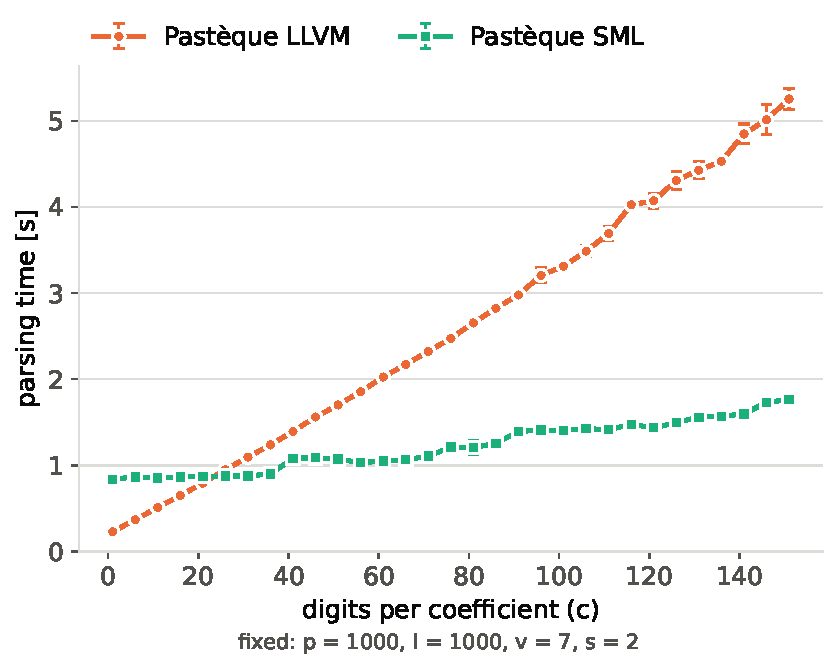
\includegraphics[width=\textwidth,height=0.75\textheight,keepaspectratio]{../evaluation/fuzzing/results/sweep-c.pdf}
        \end{column}
        \begin{column}{0.4\textwidth}
            \begin{itemize}
                \item Random input (invalid proof), evaluate parsers only
                \item All coefficients have the same length
                \item LLVM uses school-book multiplication, one multiplication per digit
            \end{itemize}
        \end{column}
    \end{columns}
    \note{
        End: 27:00
    }
\end{frame}

% \begin{frame}
%     \centering
%     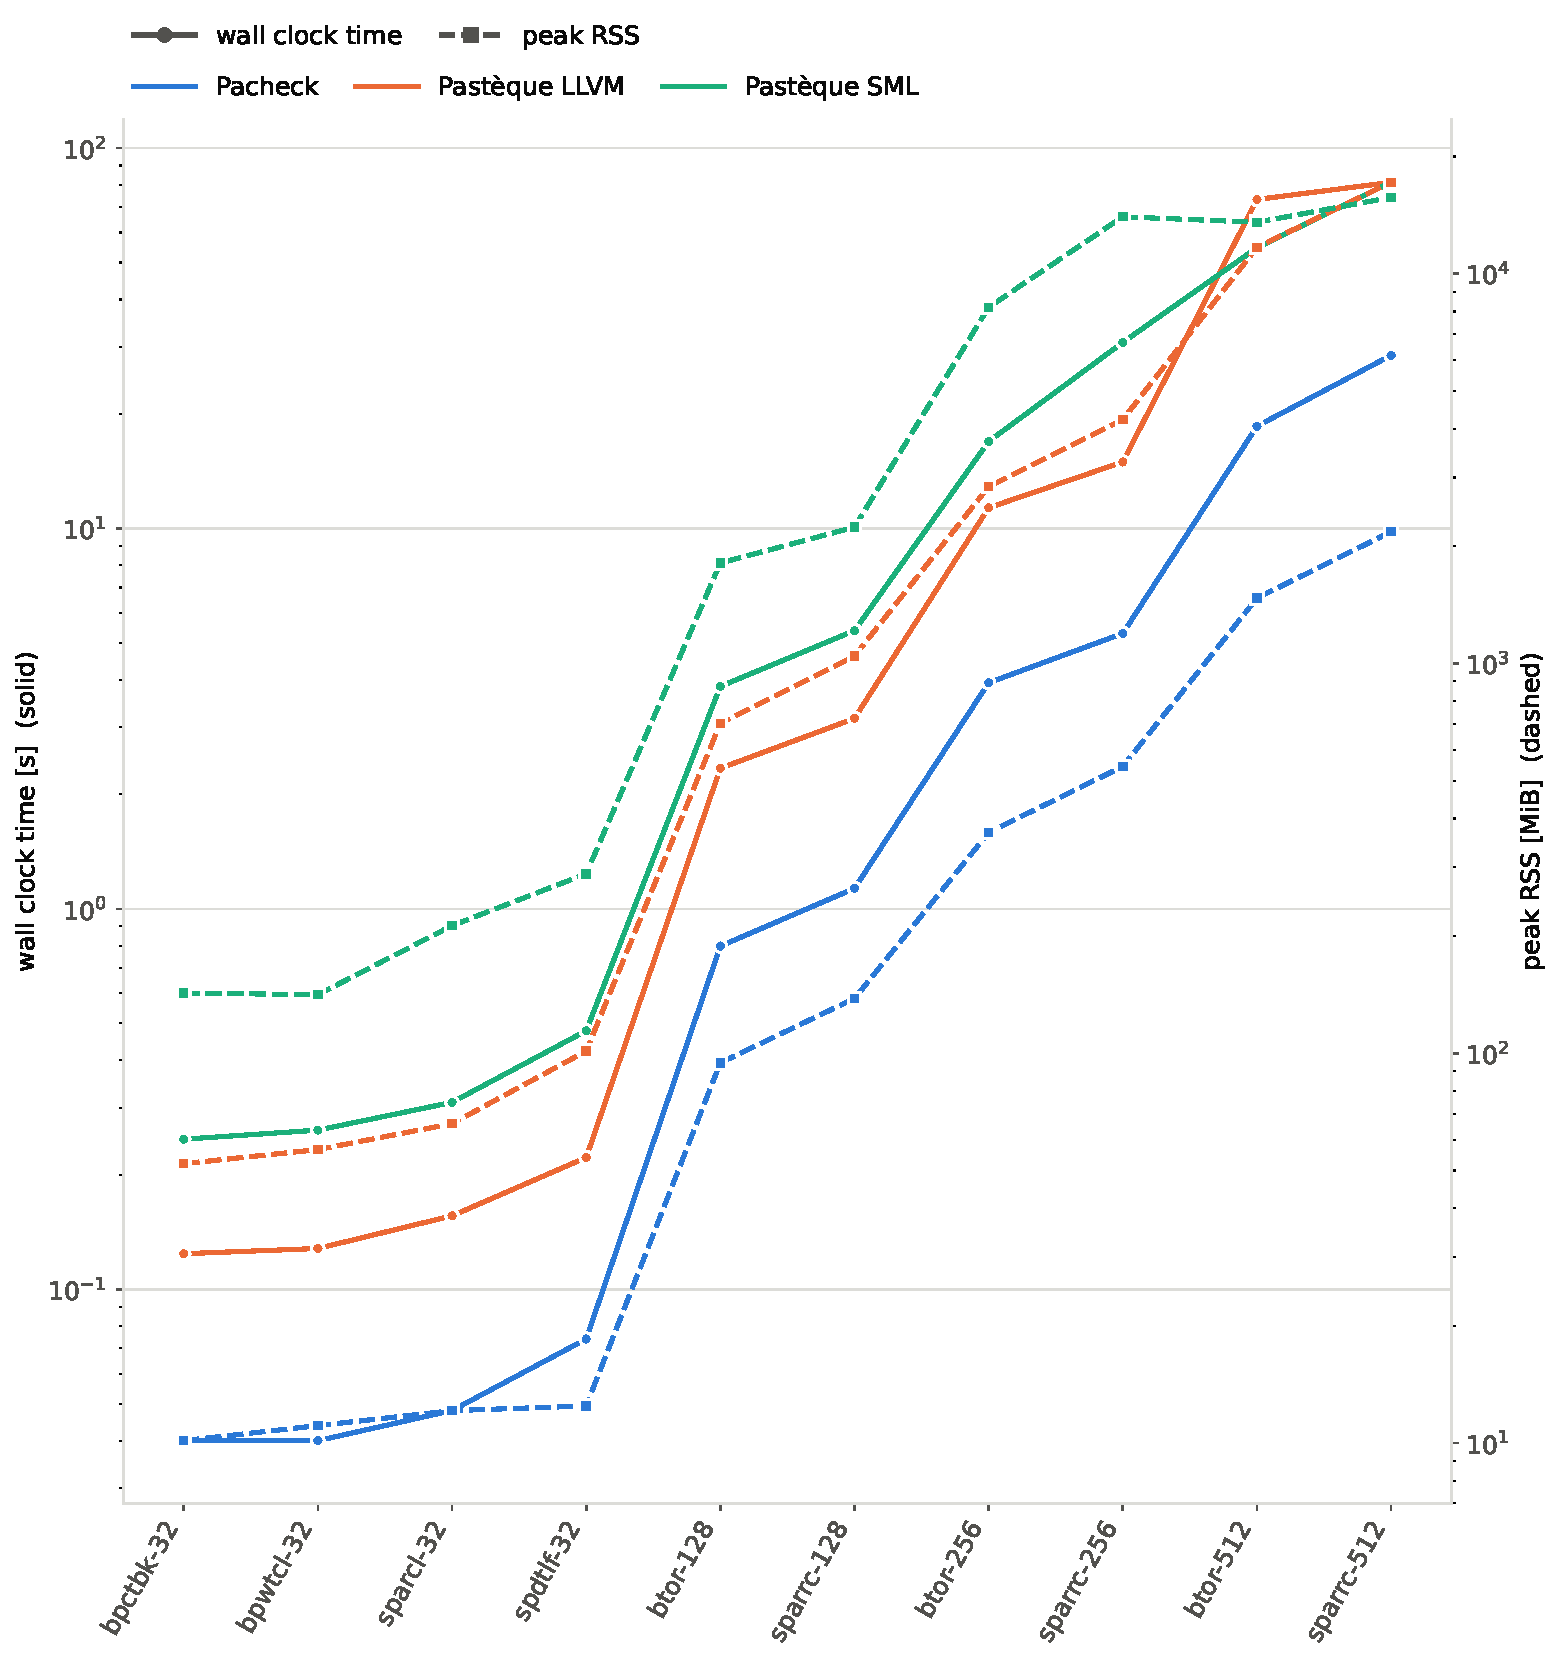
\includegraphics[width=\textwidth,height=0.85\textheight,keepaspectratio]{../evaluation/main/results/plot.pdf}
% \end{frame}

\section{Discussion}
\begin{frame}
How close can we get to Pacheck?
\begin{center}
\begin{tikzpicture}[
	var/.style={draw, rectangle, minimum width=7mm, minimum height=7mm, font=\ttfamily, text height=1.5ex, text depth=.25ex},
	heading/.style={text height=2ex, text depth=.25ex},
	ptr/.style={->, >=stealth, thick},
	node distance=6mm and 6mm,
]
% Pastèque: one separate list per term
\node[var] (pa) {a};
\node[var, right=of pa] (pb1) {b};
\node[var, right=of pb1] (pc1) {c};
\node[var, right=of pc1] (pd1) {d};
\node[var, below=of pa] (px) {x};
\node[var, right=of px] (pb2) {b};
\node[var, right=of pb2] (pc2) {c};
\node[var, right=of pc2] (pd2) {d};
\draw[ptr] (pa) -- (pb1);
\draw[ptr] (pb1) -- (pc1);
\draw[ptr] (pc1) -- (pd1);
\draw[ptr] (px) -- (pb2);
\draw[ptr] (pb2) -- (pc2);
\draw[ptr] (pc2) -- (pd2);
\node[heading, above=4mm] at ($(pa.north)!0.5!(pd1.north)$) {Pastèque};

% Pacheck: terms share their common suffix
\node[var, right=18mm of pd1] (ka) {a};
\node[var, right=of ka] (kb) {b};
\node[var, right=of kb] (kc) {c};
\node[var, right=of kc] (kd) {d};
\node[var, below=of ka] (kx) {x};
	\draw[ptr] (ka) -- (kb);
	\draw[ptr] (kb) -- (kc);
	\draw[ptr] (kc) -- (kd);
	\draw[ptr] (kx) -- (kb);
	\node[heading, above=4mm] at ($(ka.north)!0.5!(kd.north)$) {Pacheck};
\end{tikzpicture}
\end{center}
\end{frame}

\begin{frame}{Possible Improvements}
    \begin{itemize}
        \item Use fractional separation logic
        \item Terms by arrays (instead of lists)
        \item Parsing: Karatsuba Multiplication + Chunks of digits
        \item Move parsing to Isabelle side
              $\rightsquigarrow$ interleave parsing and checking
        \item Save additional pointer dereference in polynomial lookup map
    \end{itemize}
\end{frame}

\begin{frame}{AI Usage}
    \begin{itemize}
        \item Pictures in slides are AI generated
        \item Initial work on (signed) multiple precision numbers: no AI
        \item Low-level $\iexp{vcg}$ proofs - too hard (for me)
        \item Hand written definitions, AI written proofs
        \item Used Claude Code with models Opus, Sonnet and Fable
    \end{itemize}
\end{frame}

\appendix

\section{References}

\begin{frame}[allowframebreaks]{References}
    \printbibliography[heading=none]
\end{frame}

\section{Appendix}


\end{document}
